%  NOTE: Please make sure to completely fill out the \def parts in meta-data.tex!

\section*{Preface}

Foremost, I would like to express my gratitude towards all persons that helped me during the creation of this thesis. From helping me with finding the topic to helping me correct my mistakes while programming the algorithms used in this thesis. 
\\

I would like to especially thank my research supervisor \textbf{Dr. Dimitar Shterionov} (Professor at Tilburg University) for the guidance given by helping me both with the research for this topic and correcting my many mistakes while coding. 

I am grateful to my fellow Thesis colleagues \textbf{Stan van der Vossen} (CSAI-Student) and \textbf{Jakob E. Hauser} (CSAI-Student) for the advice, translating sporadic German to English, and guidance given towards solving the problems I faced during the creation of this Thesis paper.

Lastly, even though they are unaware of me writing this Thesis paper, I would like to express my gratitude towards all the researchers that aided in the creation of the DGS-Korpus and especially for making it available to the online public.

\newpage \thispagestyle{empty} \strut
\newpage \pagenumbering{arabic}

\title{\thesistitle{}}
\author{\yourname}

\maketitle % Yes, again

\begin{abstract}

Sign languages are languages that have their own unique grammar, words and manners of speaking and can be therefore completely distinct from the regional equivalent language. Most of the time they live in parallel worlds, with the deaf on one side and the hearing on another. When these worlds clash confusion arises because of the dissimilarity between the two since they might not stem from the same language family. In recent years the field of neural machine translation has grown exponentially, with the invention of the transformer architecture increasing accuracy in parallel machine translation software. German Sign Language (DGS) and German are two distinct languages and are therefore subject to translation possibilities. The recent approaches mainly focus on (German) text to (DGS) glosses. However,  there has been a lack of a glosses-to-text translation system. The focus of this paper is to find the best approach by adding temporal, vocal, or combined data to the glosses of the DGS Public Korpus. The results show that adding these extra tokens to the data results in a less accurate translation across all models. The neural machine translation system with an input of nothing but glosses [BLEU 3.69, TER 0.960] outperforms the more complex models [average BLEU 2.19, average TER 0.981]. It is concluded that adding temporal, vocal or both aids in the emergence of more rare and unique words resulting in the decrease in accuracy of the model.

\end{abstract}

\section{Introduction}

early linguistics vs early sign language study

\cite{stokoe2005sign}
sign language us actually a language

GLOSSES

zowel basic lstm en transformer

machine translation en transformers \cite{vaswani2017attention}

papers die hier precies mee te maken hebben
\cite{garcia2016factored}

basic NMT and NLP

\subsection{Research Question}

\textbf{To what extent does temporal data aid in the performance of a machine translation system for sign language glosses to text?}

\begin{itemize}
    \item \textbf{How to introduce temporal data to the Machine Translation system?} \\
    The baseline system does not have temporal data added to it. This sub-question is related to how to add temporal data to the machine translation system.
    \item \textbf{To what extent does temporal data aid a Machine Translation system when compared to a baseline system?} \\
    The chosen dataset \cite{dgscorpus_3} contains both the glosses (i.e.: TO-HAVE-BSL1, I1\textasciicircum, BUTTER1A) and the timestamps next to them to indicate when and how long these signs have taken place. This sub-question is related to combining this temporal data with the baseline system. Both the baseline and the temporal experiments are described in the methods section.
    \item \textbf{To what extent does adding extra tokens have an effect on the performance of the Machine Translation system} \\
    The dataset contains both glosses on sign language and data on what the subject said during the interview (vocal). This sub-question is related to:
    \begin{enumerate}
        \item Combining the additional vocal data with the baseline system.
        \item Combining the additional vocal data with the temporal data and the baseline system.
        \item Measure to what extent does adding extra tokens have an effect on the performance of the Machine Translation system.
    \end{enumerate}.
\end{itemize}

\section{Related Work}

Research on parallel translation of spoken language is widely attested. Sign language translation, however, is a relatively small field with little appropriate datasets or methods \cite{camgoz2021content4all} \cite{bragg2019sign}. In the late 1990s, the field of Sign Language translation wasn't much of a separate field, the research that did exist was mainly focused on recognizing sign language. The focus of Sign Language Recognition mainly relied on using HMMs (\citealp{hiddenmarkov1l}; \citealp{hiddenmarkov2}; \citealp{hiddenmarkov3}) \cite{holden2005australian} A gesture would be decomposed into a sequence of postures. These postures would then be recognised by the HMM as a gesture. For the system to be able to track a gesture the user would be wearing an annotated glove. For example, coloured rings would be worn around each finger. This approach changed in 1996 by using the colour of the participants' skin to segment from the background by calibrating the system on the participants noses \cite{starner1998real}. This proved to be problematic, however, since the hands move at a different pace compared to the nose the system would occasionally filter out the nose \cite{starner1998real}. In 2005, a end-to-end pipeline , called the Sign2 Conversion System \cite{glenn2005image}, was created. However, it was only being able to be used for ASL finger-spelling excluding any non-alphabetical ASL signs.

Using neural networks in sign recognition was among the first methods proposed at the onset of the field \cite{murakami1991gesture} \cite{fels1993glove}, however the approach was overshadowed due to the success of HMM's in the 1990s \cite{cooper2011sign}.  

The use of neural networks became more prominent in the late 2000s \cite{parton2006sign}, (\citealp{ethopia}; \citealp{malaysia}; \citealp{persia}; \citealp{brazil}; \citealp{arabia})

More recently, the field can be divided into two main trends, the  Sign Language Translation (SLT) trend and the Continuous Sign Language Recognition (CSLR) trend. Continuous Sign Language Recognition systems \cite{koller2015continuous}

vergelijk lstms vs. transfromer hier
NOG AFMAKEN!!!!!!!!

SOTA \cite{camgoz2018neural}

\section{Data}

\subsection{Source}

The data consists of $405$ EAF-files (ELAN Annotation Files) gathered by the Institute for German Sign Language and Communication of the Deaf at Hamburg University \cite{prillwitz2008dgs}. These files consist of a total of $50$ hours of annotated recordings spanning a wide range of narrations regarding the cultural aspects of the deaf community. The interviews were conducted using a peer-to-peer procedure, where participant change roles according to the conversation \cite{prillwitz2008dgs}. During a discussion $2$ German Sign Language or Deutsche Gebärdensprache (DGS) signers conversed. Each conversation consisted of a standardized interview covering linguistical and social data \cite{deaf_areas}. Following this conversation, a spontaneous conversation on a given topic was held while the participants were encouraged to use as much basic vocabulary as possible \cite{deaf_areas}. In the EAF-files the signers are annotated as either Speaker A or Speaker B. The data was collected between January $2010$ and December $2011$  by videotaping $330$ participants from all $16$ Federated States (Bundesländer). The recordings were conducted using a mobile field lab in:

\begin{itemize}
  \item Areas with a relatively high deaf population density (deaf schools, deaf centres, and deaf institutes). \cite{age_data_hamburg} \cite{deaf_areas}
  \item The catchment areas of the former Schools for the Deaf.\cite{age_data_hamburg} \cite{prillwitz2008dgs}
  \item Areas which were easy to reach from surrounding rural communities. \cite{age_data_hamburg} \cite{deaf_areas}
  \item Areas that were suspected of having a distinct dialect. \cite{age_data_hamburg} \cite{prillwitz2008dgs}
\end{itemize}

 The data was collected by representatives of the local deaf community to take into account the regional varieties of DGS \cite{deaf_areas}. As can be seen in \autoref{fig:bundeslander} the data was sampled from participants across different age groups \cite{age_data_hamburg}. 


% Age category figure
\pgfplotstableread[row sep=\\,col sep=&]{
    interval & carT & carD \\
    18--30     & 12.1  & 12.4  \\
    31--45     & 13.6 & 13.9  \\
    46--60   & 12.7 & 12.4 \\
    61+   & 11.5 & 11.2 \\
    }\mydata

\begin{figure}[h]
\caption{Showing the percentage of participants per age , divided into both the Male (shown in Purple) and Female (shown in Red) gender,  that participated in the creation of the DGS corpus (both annotated and non-annotated). \cite{age_data_hamburg}}
\begin{tikzpicture}
    \begin{axis}[
            ybar,
            title={Age distribution in The DGS-Korpus project sample (Percentage Vs. Age Categories)},
            bar width=.6cm,
            width=.8\textwidth,
            height=.5\textwidth,
            legend style={at={(0.5,1)},
                anchor=north,legend columns=-1},
            symbolic x coords={18--30,31--45,46--60,61+},
            xtick=data,
            nodes near coords,
            nodes near coords align={vertical},
            ymin=0,ymax=25,
            xlabel={\/Age categories},
            ylabel={\/Percentage of participants (\%)},
        ]
        \addplot table[x=interval,y=carT]{\mydata};
        \addplot table[x=interval,y=carD]{\mydata};
        \legend{Male, Female}
    \end{axis}
    
\end{tikzpicture}

\label{fig:bundeslander}
\end{figure}

\subsection{ELAN}
The conversation conducted between the representatives of the deaf community has been annotated and stored in EAF-files. These EAF-files can be shown and edited using the ELAN software \cite{crasborn2008enhanced}. ELAN is a multimedia annotation software developed by \citep{elan_software} to assist in Linguistical studies, language conservation, and sign language research \cite{brugman2004annotating}. The software can be used to add annotations to video and/or audio recordings. An annotation can be a sentence, word, or in the case of sign language, a gloss. Using ELAN multiple annotations can be created that are sorted into tiers \cite{crasborn2008enhanced}.  

% EAF-example
\begin{figure}[h]
\caption{Showing the structure of one of the EAF (English Annotated File)-files \cite{elan_example} inside the program ELAN. ELAN is a multimedia annotation tool used for multi-modality research \cite{sloetjes2017elan}. }
 \centering 
 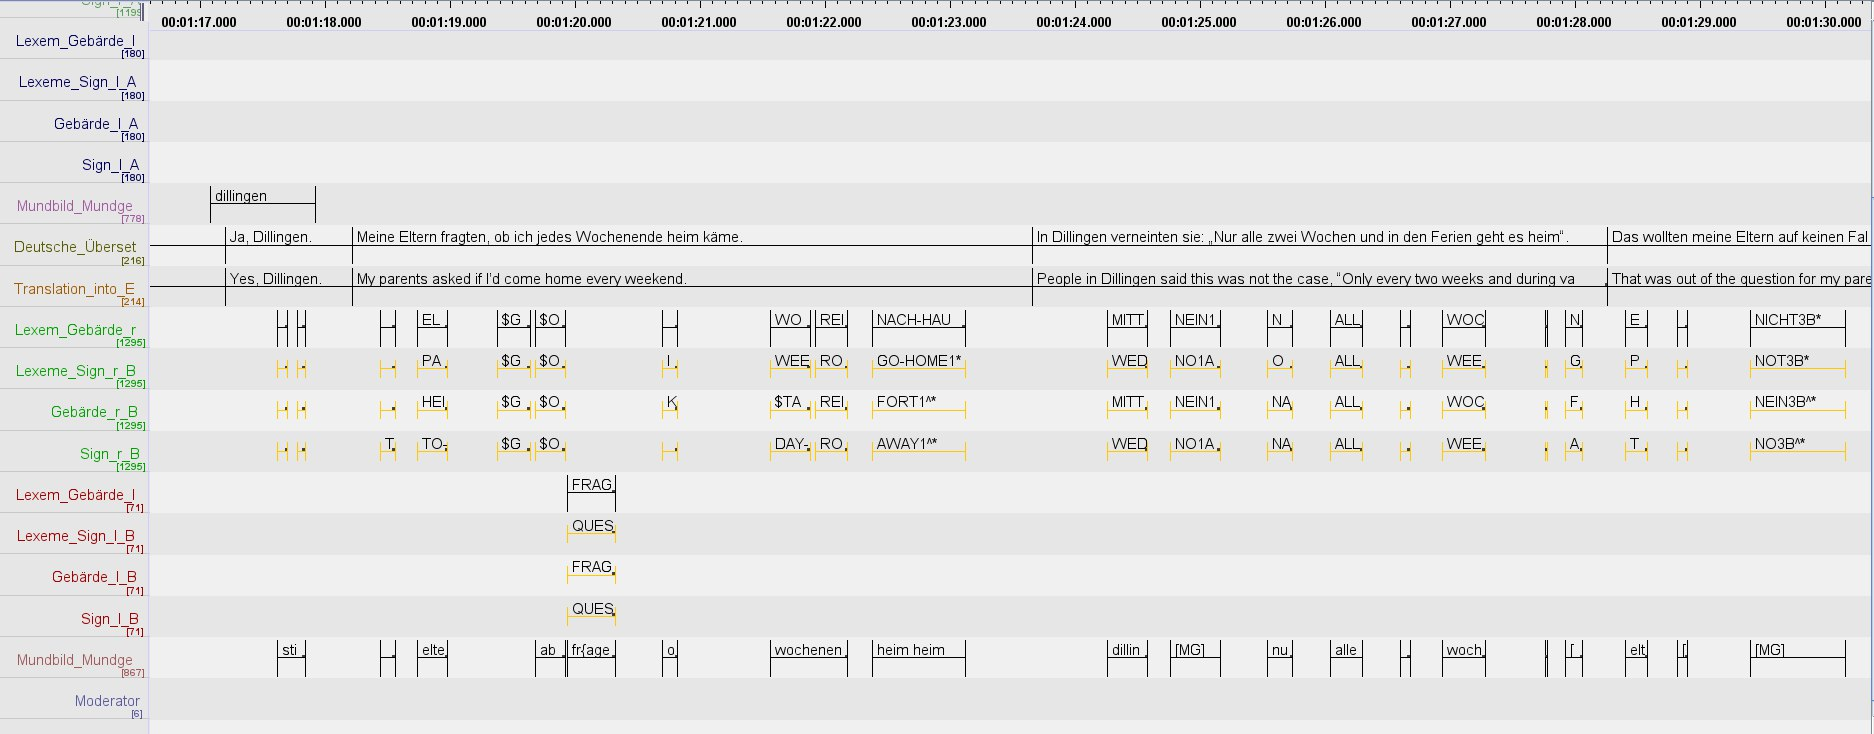
\includegraphics[width=14cm]{Bachelor CSAI thesis template/images/ELAN_example.jpg}
 
 \label{fig:elan_example}
\end{figure}

\subsection{Initial Translation}

The annotations divided into tiers are presented across a timeline. As can be seen in \autoref{fig:elan_example}these files are divided into $11$ different tiers, presented in both English and German due to accessibility \cite{konradoffentliches}. Take "Lexem\_Gebärde\_r\_A" for example, this tier is translated into English as "Lexeme\_Sign\_r\_A". The tiers present in the EAF-files, translated into English, are: "Time", "Sign\_l\_B", "Sign\_r\_B", "Lexeme\_Sign\_l\_B", "Lexeme\_Sign\_r\_B", 
"Translation\_into\_English\_B", "Sign\_l\_A", "Sign\_r\_A", "Lexeme\_Sign\_l\_A", "Lexeme\_Sign\_r\_A", and "Translation\_into\_English\_A" \cite{sloetjes2017elan}. The goal of this paper is to, through experimentation, show to what extent temporal data aids in the performance of a machine translation system for sign language glosses to text. For this purpose, both the German Sign Language and the German Language were chosen respectively. Since the target language is German it was decided to use the original glosses and translations that were available in the corpus.

The initial translation of the glosses in the data set (i.e.: Sign\_l\_A to Translation\_into\_English) was conducted by contracted sign language translators and interpreters \cite{konradoffentliches}. These researchers translated the data set word-for-word. Consequently, university students created coherent meaningful sentence like structures. Lastly, these sentences were fed back into the system until the proper meaning was determined by the DGS experts (\autoref{fig:uselesspipeline}) \cite{konradoffentliches}.

\begin{figure}[h]
\caption{Showing the translation pipeline of the initial translation phase as conducted by the Institute for German Sign Language and Communication of the Deaf at Hamburg University. \cite{konradoffentliches} }
 \centering 
 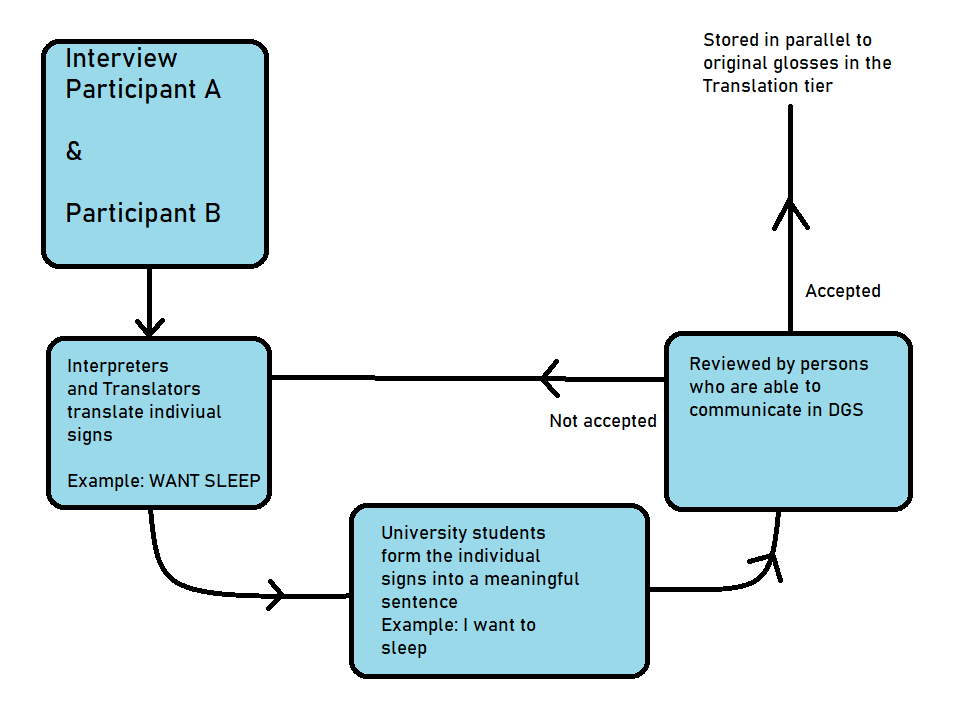
\includegraphics[width=14cm]{Bachelor CSAI thesis template/images/translation_pipeline.png}
 
 \label{fig:uselesspipeline}
\end{figure}

\subsection{Segmentation}

As with spoken languages, sign languages tend not to have a naturally occurring white space character \cite{hankesegmentation} \cite{konradoffentliches}. Thus it is difficult to determine where a sign begins and where a sign ends. In this situation, the segmentator has two options: either add a gap or none at all. Unlike spoken languages, when a participant is signing two words, take TREE (rest your right forearm upon your left palm and twist) \cite{perniss2007space} and COW (make two horns using your thumb and little finger on top of your head), for example. There is a transitional period where the participant moves his or her arm from one sign to the next. When adding a gap between the signs, the segmentator determines that the transitional movements are not part of the token's form \cite{konradoffentliches}. Taking this into account researchers at the University of Hamburg have decided that for the creation of the DGS corpus gaps will be added. The direct result of this decision is located in the EAF files, where there is temporal data with no associated annotations.

\subsection{Lemmatisation and Gloss conventions}

When creating a corpus there is an intrinsic need to have conventions in place to make sure a uniform dataset is created. \cite{konradoffentliches} Therefore it is necessary to employ linguistics to standardise glosses using gloss conventions: \cite{kristoffersen2016designing}

\begin{itemize}
    \item In the field of Linguistics or more specifically in the field of lexicography, a lexical item forms the basic element of the lexicon of a language. Lexical signs are treated as items, that is as units of their respective sign language that would be found in the dictionary \cite{konradoffentliches}. When a deaf person signs SQUARE1\textasciicircum  it may mean different things such as a map, a recipe, or a page. In DGS \cite{perniss2007space} and several other European Sign Languages signs are iconically motivated \cite{pietrandrea2002iconicity} \cite{oomen2017iconicity}, meaning that there is a similarity between the form of the sign and the meaning of the sign. In the DGS corpus, type glosses are given an indication of iconic value by using a circumflex at the end: "SQUARE1\textasciicircum ". Examples of child types to the SQUARE1\textasciicircum parent type are: FORM1, MIRROR2, and PAPER4, these and all other non-circumflex glosses are subtypes. The numbers denote different lexical variants.
    \item Fully iconically motivated signs, also known as poly-morphemic signs, are denoted as productive signs in contrast to lexical signs that denote something instead of meaning. Productive signs, therefore, have a \$PROD token \cite{konradoffentliches}
    \item Due to the anonymisation laws present in Germany, where this corpus was created, all names are replaced by "\$NAME". Except when it concerns a famous person the \$NAME gloss is followed by the person's name. \cite{konradoffentliches}
    \item Foreign language elements are represented using the INTS token, for example, when signing the English word Germany instead of "Deutschland" it has been written as GERMANY-INST1.\cite{konradoffentliches}
    \item In German Sign Language it is conventional to use a one-handed manual alphabet, for example when spelling out someone's name. For these situations, the \$ALPHA token is used. Numbers are presented similarly by using \$NUM. \cite{konradoffentliches}  
\end{itemize}

Taking into account these points a uniform corpus was created with annotated signs presented on a timeline. An example of an annotated DGS sentence can be seen in \autoref{fig:sentence_example}.

\begin{figure}[h]
\caption{Showing an example sentence of the annotated corpus in DGS glosses. The German translation of this gloss sentence is: "Und dann fällt es einem wieder auf, dass der andere noch Fehler macht" \cite{dgscorpus_3}. (English translation: And then one notices again, that the other (person) is still making mistakes). 1. A token denoting a gesture. 2. The sign annotated as NM has iconic meaning. 3. One of several lexical variants of the lexical unit FEHLER.}
 \centering 
 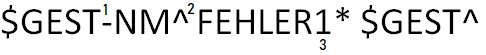
\includegraphics[width=14cm]{Bachelor CSAI thesis template/images/sentence_example.png}
 
 \label{fig:sentence_example}
\end{figure}

\section{Methods}

\subsection{Experiments}

To answer the (sub-) research questions, experiments are needed. Described below are $4$ experiments that have been designed to test the hypotheses, they differ mainly in data structure. A good overview of their differences can be found in (\autoref{fig:baseline_comparison}). 

\subsubsection{Baseline}

To the baseline the other experiments will be compared. This model lacks any external added tokens. It consists of the glosses formed into a sentence as the source and their German translations as the target (Source: PRIVAT1A* FAMILIE1 Target: Privates oder Familie? \cite{dgscorpus_3}). The sign language glosses are without any transitional periods (See the Lemmatisation and Gloss conventions section in Data) and adhere to the standard gloss conventions.


\subsubsection{Temporal}

A sub-goal of this thesis-paper is to, through experimentation, show to what extent temporal data aids in the performance of machine translation systems for sign language glosses to text. This will be tested in the Temporal experiment. The data in the temporal experiment consists of the glosses formed into a sentence with tokens added to each word separated by a "|" character, e.g.: FAMILIE|120. The number behind the "|" character represents the total amount of milliseconds it took for a sign to be signed, in the given example this would mean that the sign for FAMILIE (English: Family) would have taken 120 ms to be made. As mentioned before these sentences are without the transitional periods from one sign to another (See the Lemmatisation and Gloss conventions section in Data). The "|" sign is a library standard sign to split Word features from the actual words \cite{klein-etal-2017-opennmt}. The temporal data files consist of glosses formed into a sentence with added temporal data and their German translation as the target (Source: PRIVAT1A*|340 FAMILIE1|460 Target: Privates oder Familie? \cite{dgscorpus_3})

\subsubsection{Vocal}

Another sub-goal of this thesis paper is to show to what extent adding extra tokens aids in the performance of machine translation systems for sign language glosses to text. This will be tested in both the Vocal and the Combined experiment. The data in the vocal experiment consists of glosses formed into a sentence with tokens added to each word that represent the spoken words uttered by the participant while performing this sign. Research has shown that the mouthing a deaf-person performs is of importance for the meaning of the sign that is being performed at the same time \cite{kristoffersen2016designing}. The spoken word and the gloss will be separated by the "|" character as per library standard \cite{klein-etal-2017-opennmt}. When using the OpenNMT library \cite{klein-etal-2017-opennmt} it is necessary that all source word features have the same amount of features. Thus when a sign does not have an accompanied mouthing a "nan" will be added instead of the spoken word. This is done to represent the empty space created by the empty row. The vocal data files consist of glosses formed into a sentence with added vocal data and their German translation as the target (Source: PRIVAT1A*|privat FAMILIE1|familie Target: Privates oder Familie?). It is important to note that all vocal word features are denoted solely using lowercase characters.

\subsubsection{Combined}

Research has shown that talking speed is affected by emotions \cite{kshirsagar2002multilayer}. The combination experiment is an experiment that combines the previously mentioned temporal and vocal features into one model.  The data will be seperated by a "|" and be processed in a GLOSS|vocal|TIME format. The same conditions apply on the combined model as applied on the vocal and temporal model. The combined data files consist of glosses formed into a sentence with added vocal and temporal data and their German translation as the target (Source: PRIVAT1A*|privat|340 FAMILIE1|familie|460 Target: Privates oder Familie? \cite{dgscorpus_3}).

\begin{figure}[h]
\caption{Showing the source file textual comparison between the Baseline, Temporal, Vocal, and Combined experiments. In the temporal experiment the concept of time is added (in ms). In the vocal experiment the concept of spoken words is added (in lowercase letters). In the combined experiment these are combined into one.}
 \centering 
 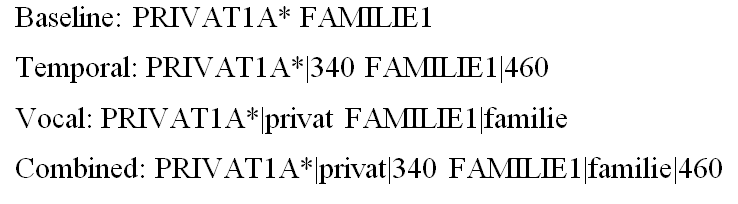
\includegraphics[width=14cm]{Bachelor CSAI thesis template/images/baseline_compared.PNG}
 
 \label{fig:baseline_comparison}
\end{figure}


\subsection{Pre-Processing}

\subsubsection{EAF to CSV}
Using the ELAN software $7$ of the $11$ tiers were selected and converted into a CSV file. This creates $2$ distinct CSV files that were consequently merged (\autoref{apx:first}). Due to having merged the files, there are no longer multiple persons in the data set, instead, the data set has transformed into a contextless database. Due to being able to access the timeline in ELAN \cite{elan_software}, it is possible to extract the temporal features of a given annotation. As mentioned before the annotators decided to add gaps between the signs \cite{hankesegmentation} \cite{konradoffentliches}, this has been carried over into the EAF-files, resulting in empty rows inside the CSV file. These need to be removed since the program automatically puts white spaces between words instead of pasting them into one giant string (\autoref{apx:first}). Failing to do so would result in temporal features being assigned to empty strings (A temporal-annotated sentence without removal of prior white spaces would result in \$GEST-NM\textasciicircum|430 |230 FEHLER1*|450 |400 \$GEST\textasciicircum|400).

\subsubsection{Data splitting}

After merging the data, the dataframe contains $5$ columns. As has been described $4$ experiments are to be performed: Sign, Temporal, Vocal, and Combined. For each of these experiments two files are need: a Source file (.src) , and a Target file (.trg). These files are fully extracted from the dataframe. By isolating the sentences in the dataframe it is possible to create a separate sentence set for every sentence. This will result in $5$ files: normal.en, vocal.en, times.en, combined.en and sentences.nl. "sentences.nl" is the target file for all the experiments and is therefore uniform.

To tokenize and split the data the \texttt{train\_test\_dev.py} (SOURCE NEEDED) script was used to both tokenize and split the data into a training, a validation, and a testing file. Since the data set only has $60000$ sentences it was decided to split the data into only 500 sentences for validation and testing each while the remaining $58000$ sentences were used for the training file.

An unwanted side-effect of the \texttt{train\_test\_dev.py} script is that it adds white spaces between the individual sentences in both the (train, test, dev) source files as the target files. This results in the Machine Translation system "assigning" sentences to these white spaces when training, resulting in a normal German sentence within a normal German sentence. For this reason all files are passed through the \texttt{remove\_whitespace.py} script (\autoref{apx:fixing}) which will strip away all empty lines. Applying \texttt{remove\_whitespace.py} on the data files significantly increases the BLEU-score for the Baseline model, while the old Baseline (pre-BPE, pre-fixing) had a BLEU score (See the section on BLEU-score for more details) of 1.36 the new Baseline (pre-BPE, post-fixing) had a BLEU score of 2.15, it was therefore decided to use the \texttt{fixing.py} on all data files.


\subsubsection{BPE}

Byte Pair Encoding (BPE) is a general-purpose data compression algorithm \cite{sennrich2015neural} \cite{gage1994new}. The way it works is by replacing the most frequent pair of bytes in a sequence with unused bytes, in the case of the OpenNMT Byte Pair Encoding \cite{klein-etal-2017-opennmt} scripts the unused bytes were denoted in the data files as "@@ ". The advantages of using the BPE algorithm are:

\begin{enumerate}
    \item \textbf{Memory}. In the case of German, many words start with the unit "auf", by encoding this unit by only using $1$ symbol, the system only encounters one symbol instead of $3$. \cite{gage1994new}
    \item \textbf{Out-of-vocabulary words (OOV)}. Taking into account the previous example, since the unit "auf" has been replaced by $1$ symbol encountering it will be familiar. This is because BPE allows for the encoding of rare words and will not introduce any unrecognised tokens. \cite{gage1994new} \cite{sennrich2015neural}
\end{enumerate}

Before being passed to the pre-processing and training, the data, except for the test.trg-file, was passed through a modified form of the BPE-algorithm. In normal circumstances when using BPE it causes no problems, however, when applying BPE to data containing word features it will split the word on the "|" character. The modified algorithm first double checks whether or not there is a temporal feature added to the word and if there is will join the word and its respective temporal feature together (\autoref{apx:bpemod}). Applying \texttt{fixing.py} on the data files significantly increases the BLEU-score for the Baseline model, while the old Baseline (pre-BPE, post-fixing) had a BLEU score 2.15, the new Baseline (post-BPE, post-fixing) had a BLEU-score of 3.69. It was therefore decided to use the Byte Pair Encoding algorithm to compress the data files.


\subsection{OpenNMT}
 
To train the data a library is needed that both support Neural Machine Translation and support source word features. With these criteria in mind $2$ libraries were eventually found: OpenNMT \cite{klein-etal-2017-opennmt} and MarianNMT \cite{mariannmt}. A main difference between the two remaining libraries is the way source word features can be used. Consider the following sentence: "PRIVAT1A*|340 FAMILIE1", as can be seen the first word has a word features attached, however, the second word does not. While this is not a problem in MarianNMT this would be a cause a problem in OpenNMT since it source word features need to be consistent. Nonetheless, OpenNMT was chosen as the preferred library because of its compatibility with Microsoft Windows $10$.

\subsection{Hyperparameters and Architecture}

Using the OpenNMT library \cite{klein-etal-2017-opennmt} a model was trained on the Transformer architecture. The hyperparameters were picked to match the recommended standard transformer hyper-parameters \cite{standard_hyperparameters} as shown in (\autoref{tab:parameter}). These settings were chosen as to create a model that is able to imitate the WMT2014 German-English \cite{WMT2014} results as achieved by the original paper on Transformers \cite{vaswani2017attention}. Overfitting on a small data set (the training data consists of $60000$ sentences) is a major challenge \cite{barone2017regularization}, therefore,  an early stopping criteria was introduced. If the perplexity and accuracy of the model do not improve during the last 5 validation performances the system will be stopped. Due to the limited capabilities of the system used, even with the use of the BPE algorithm, the batch size had to be decreased from a recommended 4096 to 1024.



\begin{table}[h]
\caption{Showing the hyperparameters used for training using the Transformer architecture. It is important to note that the  }
\centering
\begin{tabular}{|ll|ll|}
\hline
\multicolumn{1}{|l|}{Hyperparameter} & Setting     & \multicolumn{1}{l|}{Hyperparameter} & Setting              \\ \hline
Encoder type                    & Transformer & Batch size                     & 1024                 \\
Decoder type                    & Transformer & Batch type                     & tokens               \\
Transformer feed-forward        & 2048        & Normalization                  & tokens               \\
Layers                          & 6           & Warm-up steps                  & 8000                 \\
Heads                           & 8           & Training steps                 & 20000                \\
RNN size                        & 512         & Validation steps               & 1000                 \\
Word embedding size             & 512         & Label smoothing                & 0.1                  \\
Position encoding               & True        & World size                     & 1                    \\
Maximum generator batches       & 2           & GPU rank                       & 0                    \\
Dropout probability             & 0.1         & Early stopping                 & 5                    \\
Optimization method             & adam        & Early Stopping criteria        & perplexity, accuracy \\
Adam beta2 hyperparameter            & 0.998       & Max gradient norm              & 0                    \\
Decay Method                    & noam        & Parameters initialized at      & 0                    \\
Learning rate                   & 2           & Parameters\_init\_glorot       & True                 \\ \hline
\end{tabular}

\label{tab:parameter}
\end{table}

\subsection{BLEU}

BLEU is short for Bilingual Evaluation Understudy and is an evaluation metric for Neural Machine Translation as described in \cite{papineni2002bleu}. As the name suggest it is a evaluation metric for a parallel bilingual system with a reference (original target file) and a hypothesis (predicted target file). Previously used metrics were human-based and could take weeks or even months to be calculated \cite{papineni2002bleu}. Thus BLEU was created, the idea behind the metric is that the closer a machine translation is to a professional (linguistic) human translation, the better it is. Therefore one has to measure how close the prediction is to the reference translations.

\subsubsection{Weighted precision}
BLEU makes use of the weighted precision score (\autoref{fig:weighted_precision}). The difference between the modified version and the normal version is that the modified version takes into account the maximum reference count \cite{chan}. If using multiple references the "normal" precision measure was used the sentence "dog dog dog dog dog dog dog" would be able to get a score of 1. This is especially true since Machine Translation systems tend to over-generate words that seem to fit in \cite{papineni2002bleu}.

\begin{figure}[h]
\caption{Showing the modified n-gram precision formula. The difference between the modified version and the normal version is that the modified version takes into account the maximum reference count, known as the clipped count. Candidates refers to the translated sentences \cite{chan} \cite{papineni2002bleu}. First compute the N-gram matches. Second add the clipped counts for all translated sentences. Third divide the sum by the total number of n-grams in the reference. \cite{chan}}
 \centering 
 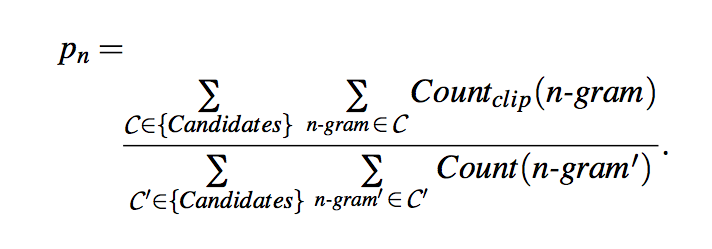
\includegraphics[width=10cm]{Bachelor CSAI thesis template/images/weighted_precision.png}
 \label{fig:weighted_precision}
\end{figure}

\subsubsection{Brevity penalty}
Although not applicable in this paper, traditionally the BLEU-score was used to calculate the score of a prediction over multiple references. Since these references may or may not have variable length this will negatively affect the recall score \cite{papineni2002bleu} (Section 2.2). The proposed solution is the brevity penalty or BP for short as can be seen in (\autoref{fig:full_bleu}). The Brevity penalty high scoring translations must match the references in word order and length. Sentences smaller than the reference sentences are therefore penalized since they are multiplied by a factor < $1$. 


\begin{figure}[h]
 \caption{Showing the complete formula for calculating BLEU \cite{papineni2002bleu}. In the BP formula, c denotes the total length of the translation corpus, r is the sum of the best match lengths of the translation sentence in the test corpus \cite{papineni2002bleu}. If the BP value is 1 this means that the translation length and the reference length are equal if this is not the case the second formula will be used. The eventual BLEU-score is the average of the weighted precision scores times the brevity penalty, and therefore penalizes shorter sentences. }
 \centering 
 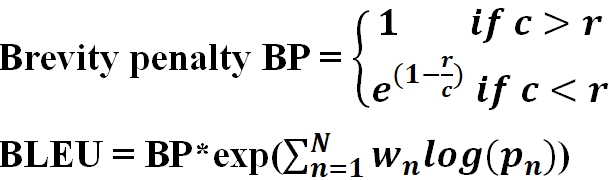
\includegraphics[width=8cm]{Bachelor CSAI thesis template/images/bleu_formula.PNG}
 \label{fig:full_bleu}
\end{figure}

\subsubsection{BLEU-score}

The BLEU score ranges from 0 to 1, with 0 being absolutely not related to the reference sentence and 1 being identical. As a convention in the field of Neural Machine Translation, the BLEU-score is either multiplied by 10 or 100, for the purposes of this paper the BLEU-score will be multiplied by 100. For the purposes of this paper BLEU will be used on only $1$ reference since there is only one available per gloss sentence.

\subsection{TER}

Translation Edit Rate (TER) measures the amount of editing that needs to be done to create an output that exactly matches a reference translation \cite{TERsnover2006}. There can be multiple TER-scores since it may match one of the references, however, since in this paper only one reference will be used this will not be considered a problem. The higher the TER-score the worse the translation, since the more edits on the total edits it needs to perform the closer it comes to $1$. The formula to calculate the TER-score is shown in (\autoref{fig:full_ter}). The number of edits is calculated in two different phases \cite{shapira2002edit}:
\begin{enumerate}
    \item A greedy search algorithm is used to find the words that need to be shifted from one place to another.
    \item An optimal calculation is made to calculate the smallest amount of remaining edits (insertion, deletion, and substitution) necessary to match the reference.
\end{enumerate}



\begin{figure}[h]
 \caption{Showing the formula for calculating the TER score \cite{TERsnover2006}. The TER-score is calculated by dividing the number of edits by the average number of words in the reference translation. Possible edits are: insertion, deletion, substitution, and switching words around. All these edits have an equal cost.}
 \centering 
 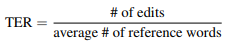
\includegraphics[width=7cm]{Bachelor CSAI thesis template/images/ter_formula.PNG}
 \label{fig:full_ter}
\end{figure}



\section{Results}

At the beginning of this paper it was hypothesised that with the insertion of temporal data into the baseline data, there would be an improvement regarding the accuracy rate of model. Additionally it was hypothesised in a sub-hypothesis that the addition of a vocal token would increase the accuracy of the model (See Section 4.1.3 on the scientific background). For these reasons $4$ experiments were set up, the baseline, temporal (baseline + time), vocal (baseline + vocal), and combined (baseline + vocal + time). 

say what the table and figures show

talk about the improvement with the preprocessing of the baseline
talk about the standardization experiment

talk about the ter score staying the same and possibly why

talk what is going on in the graphs

geef voorbeelden van de vertalingen

\begin{table}
    \caption{Best performing models with the accompanying BLEU- and TER-scores. Highlighted in bold are the best results. As can be seen in the table the baseline outperforms all other models.}
    \label{tab:results}
    \begin{tabular}{llrr}
        \toprule
                                                                  
        Word-Form                   &  Models                           &  BLEU                & TER    \\ 
        \midrule
        \multirow{3}{*}{Original}  &  Baseline                              &   \textbf{3.69}      &  \textbf{0.960} \\
                              & Temporal                                &   2.85               &  0.971 \\
                              & Vocal                                   &   2.03               &  1.000 \\
                              & Combined (Temporal + Vocal)             &   1.69               &  0.973 \\
    
        
    \end{tabular}
    
\end{table}

\pgfplotstableread[row sep=\\,col sep=&]{
    Model &      carT         \\
    Baseline     & 3.69  \\
    Temporal     & 2.85  \\
    Vocal   & 2.03       \\
    Combined   & 1.69    \\
    }\mydata

\begin{figure}[h!]
\caption{Showing the results from the $4$ performed experiments. On the X-axis the different models are presented. On the Y-axis the score is shown, the calculation and description of the BLEU score is described in Section 4.5)}
\begin{tikzpicture}
    \begin{axis}[
            ybar,
            title={Experimentation Results (BLEU-Score vs. Model)},
            bar width=.6cm,
            width=.8\textwidth,
            height=.5\textwidth,
            legend style={at={(0.5,1)},
                anchor=north,legend columns=-1},
            symbolic x coords={Baseline, Temporal, Vocal, Combined},
            xtick=data,
            nodes near coords,
            nodes near coords align={vertical},
            ymin=0,ymax=4,
            xlabel={\/Models},
            ylabel={\/Score},
        ]
        \addplot table[x=Model,y=carT]{\mydata};
        \legend{BLEU-score}
    \end{axis}
    
\end{tikzpicture}

\label{fig:results_graph}
\end{figure}


\pgfplotstableread[row sep=\\,col sep=&]{
    Model &      carD         \\
    Baseline     & 0.960  \\
    Temporal     & 0.971  \\
    Vocal   & 1.000       \\
    Combined   & 0.973    \\
    }\mydata

\begin{figure}[h!]
\caption{Showing the results from the $4$ performed experiments. On the X-axis the different models are presented. On the Y-axis the score is shown, the calculation and description of the Translation Error Rate is described in Section 4.6}
\begin{tikzpicture}
    \begin{axis}[
            ybar,
            title={Experimentation Results (TER-score vs. Model)},
            bar width=.6cm,
            width=.8\textwidth,
            height=.5\textwidth,
            legend style={at={(0.5,1)},
                anchor=north,legend columns=-1},
            symbolic x coords={Baseline, Temporal, Vocal, Combined},
            xtick=data,
            nodes near coords,
            nodes near coords align={vertical},
            ymin=0.9,ymax=1.05,
            xlabel={\/Models},
            ylabel={\/Score},
        ]
        \addplot table[x=Model,y=carD]{\mydata};
        \legend{TER}
    \end{axis}
    
\end{tikzpicture}

\label{fig:results_ter}
\end{figure}


\section{Discussion}
waarom zijn de resultaten er wat is de hypothesis iets meer analytical
Challenges/problems

What are your trial and errors

answer research question, hypothese

gebarentaal dialect neit meegomen

schrijf een stuk over wat er gebeurt als je dat hele ding standardised

alternative bpe

eerst mariannmt dna opennmt



\section{Conclusion}

\section{Self-Reflection}

%In the first semester of the third year I decided to pick a minor course called: Software Engineering for CSAI. The main part of this course was a large project on machine translation, integration into webservers, and general software engineering practices. Out of pure coincidence it turned out that I had the best GPU. This didn't matter in the end since I switched to Google Colab. Therefore, I was assigned to work mainly on the machine translation part and came to be quite interested in it. When it was time to pick a thesis coordinator, I took the opportunity to continue this interest into my Thesis.

%\subsection{Planning}

%The project was on my part poorly planned from the start, I didn't actually start thinking about what my thesis objective would be until a good $2$ weeks into the semester. In comparison, my other colleagues had thought about it in a structured way at that point. In hindsight I should have started to think about a objective way sooner, this would save me from problems further down the road. Mainly those to do with datasets. 

%\subsection{Datasets}

%Due to my initial poor planning I started rather late with the project, literature review and dataset searching. While I thought that I had found a dataset (NGT Nijmegen Dataset, NGT -> Dutch) and wrote my bachelor thesis proposal with that dataset in mind. I would not find out until early April that this dataset was in fact not (fully) available to the public. Therefore, I had to look for a new dataset. This could have all been avoided if I was more persistent when it came to obtaining the original Dutch dataset, I should have send an e-mail instead of just giving up. Secondly, if I had started looking for a dataset sooner, this could all have been avoided. From these mistakes I learned that I should be more steadfast when it comes to problems I encounter.

%\subsection{Flexibility}

%A major setback in during the Thesis is the end of Google Colab's $12$ hour runtime. Originally I used the MarianNMT library in Google Colab to train my models like I trained my models during the course Software Engineering. However, in March of 2021 Google added a CAPTCHA function to Google Colab to check if you were still active, aside from that if you were found to not be active in that time you were banned from using their GPU's for a unknown time. Therefore, I had to switch to a local system with OpenNMT in the beginning of May, effectively starting over again. I should have looked for alternatives earlier since I was aware of this problem mid-April.

%\subsection{Paper}

\newpage
\bibliography{mybib}

\newpage
\appendix

\appendixsection{Merging Code} \label{apx:first}
\begin{lstlisting}[language=Python, caption=Shown is the Python code to merge the multiple CSV-files into one DataFrame.]
class create_file(object):
    def __init__(self, path="datasets/"):
        self.path = path
        self.inputs = listdir(str(path))
        self.dataframe = self.drop_empty()

    def clean_dataframe(self, dataset):
        """
        Load the dataset into a frame, delete the "Unnamed" column,
        and replace all instances of nothing with a numpy nan.
        Requires the numpy library.

        :param dataset: str, input name of the dataset.csv
        :return: dataframe, a cleaned dataframe with only used columns
        """
        dataframe = pd.read_csv(self.path + str(dataset), sep=",")  # Read into a frame
        dataframe = dataframe.loc[:, ~dataframe.columns.str.contains("^Unnamed")]  # Drop the "^Unnamed" column
        dataframe.replace("", np.nan, inplace=True)  # Replace the empty values with a nan

        return dataframe

    def merge(self):
        """
        The EAF-files consist of different persons, this functions merges those
        into one dataframe.

        :return: Dataframe. A merged dataframe consisting of all users.
        """
        combined = pd.DataFrame()
        for dataset in self.inputs:
            temp = self.clean_dataframe(dataset)

            # Normalize the column names into the translated versions.
            column_list = list(temp.columns)
            normalized_names = ["Time", "Right", "Mouth", "Translation", "Left"]
            # A dictionary is created with the corresponding column_list name and the normalized name
            translation_dict = {column_list[n]: normalized_names[n] for n in range(len(normalized_names))}
            temp = temp.rename(columns=translation_dict)

            # Combine the dataframes into one universal dataframe
            combined = combined.append(temp, ignore_index=True, sort=False)

        return combined

    def list_definer(self, input_list):
        """
        Finds the True instances in a list and stores their indexes.

        :param input_list: list, a list of True's and False's.
        :return: list, the list of indexes that were true in the input_list.
        """
        output_list = []
        # Looping over a enumerated input_list
        for number, element in enumerate(input_list):
            # If the element is True append the index else continue the loop
            if element:
                output_list.append(number)
            continue
        return output_list

    def drop_empty(self):
        """
        Dropping the empty rows from the dataset causing it to become more information packed.
        Downsides of this approach can be found in the Discussion of the written Thesis.

        :return: dataframe, a dataframe where there are no empty rows.
        """
        combined = self.merge()

        # Find the empty rows for each respective token (time excluded since it is always present).
        left_sign = set(self.list_definer(list(combined['Left'].isnull().values)))
        right_sign = set(self.list_definer(list(combined['Right'].isnull().values)))
        mouth_token = set(self.list_definer(list(combined['Mouth'].isnull().values)))

        # Find the intersection of these tokens.
        signs = left_sign.intersection(right_sign)
        empty_rows = signs.intersection(mouth_token)
        signs_missing = list(empty_rows)

        # Dropping the empty rows
        final_dataframe = combined.drop(signs_missing)

        return final_dataframe
\end{lstlisting}
 \break
\appendixsection{Fixing} \label{apx:fixing}
\begin{lstlisting} [language=Python, caption=Shown is the Python code to fix the false white lines created by the train\_test\_dev.py script.]
def fixing():
    """
    Fixes files by removing the extra \n that was created during the train_test_dev.py splitting of the data. OpenNMT
    does not handle empty lines well and will assign "translations".
    """
    # Get current working directory
    working_directory = str(os.getcwd())

    # Calculate the total amount of files in the working directory
    dataset = os.listdir(str(working_directory))
    total = len(dataset)

    print("\nDeleting white spaces in files\n")

    # Source (regarding the lines of code related to the tqdm-libary):
    # DDGG. (2018, Feb 22) tqdm not showing bar. Stackoverflow.com.
    # https://stackoverflow.com/questions/48935907/tqdm-not-showing-bar

    with tqdm(total = total) as pbar:
        for element in dataset:
            # Create new name
            new_name = "f-" + element
            with open(str(element), "r", encoding="utf-8") as f:  # Read from this file
                with open(str(new_name), "w+", encoding="utf-8") as fixed:  # Write in this file
                    # Removing all the extra white spaces
                    while True:
                        line = f.readline()
                        if line == "":
                            break
                        if line == "nan\n":
                            continue
                        if not line.isspace() and line != "nan":
                            fixed.write(line)
            pbar.update(1) # Update pbar by 1
\end{lstlisting}

\appendixsection{BPE Modification} \label{apx:bpemod}
\begin{lstlisting}[language=Python, caption=Shown is the Python code that is a modification to the normal Byte Pair Encoding algorithm.]
            #############
            # Normal
            #############
            for item in new_word[:-1]:
                output.append(item + self.separator)
            output.append(new_word[-1])


            ##############
            # EDIT 11/05/2021 Gijs Thissen
            # This is to "fix" the problems I am having with DGS glosses with features that get split up
            # Run code above for the normal way
            ##############
            # If new_word contains more than one element (having one element suggest there not being a temporal feature)
             if len(new_word)>1 and new_word[-1][-1].isdigit(): # Last element of last element of new_word is digit
                 for item in new_word[:-1]:
                     output.append(item + self.separator + new_word[-1])
             else:
                 for item in new_word[:-1]:
                     output.append(item + self.separator)
                 output.append(new_word[-1])
\end{lstlisting}